% A sentinel — the standing armoured guard. Nothing about it moves except what
% it is holding, which is the whole idea: this family fights entirely out of
% its gear, so the figure is a rack for gear with a helmet on top.
%
% Written by filling in tikz_figure_prompt.md.
\documentclass[tikz,border=4pt]{standalone}
\usetikzlibrary{calc}
% Colourway, overridden per creature on the pdflatex command line.
\providecommand{\Main}{6E7278}
\providecommand{\Dark}{43464B}
\providecommand{\Accent}{D3A05A}

\newcommand{\Unit}{0.055cm}
\newcommand{\Edge}{2.2pt}
\newcommand{\Rivets}{4}        % down each side of the cuirass
\newcommand{\ShoulderR}{7}

\definecolor{main}{HTML}{\Main}
\definecolor{dark}{HTML}{\Dark}
\definecolor{accent}{HTML}{\Accent}
\definecolor{ink}{HTML}{101018}

\begin{document}
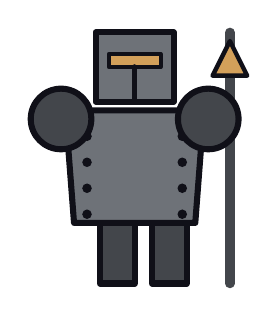
\begin{tikzpicture}[x=\Unit,y=\Unit, line join=round, line cap=round]

  % ---- the haft, behind everything ---------------------------------------
  \draw[dark,line width=3.4pt] (52,2) -- (52,60);
  \fill[accent,draw=ink,line width=1.6pt] (52,58) -- (48,50) -- (56,50) -- cycle;

  % ---- legs ---------------------------------------------------------------
  \foreach \x in {22,34} {
    \fill[dark,draw=ink,line width=\Edge] (\x,2) rectangle ++(8,16);
  }

  % ---- cuirass ------------------------------------------------------------
  \fill[main,draw=ink,line width=\Edge] (16,16) -- (44,16) -- (46,42) -- (14,42) -- cycle;
  \foreach \i in {1,...,\Rivets} {
    \pgfmathsetmacro\y{18+(\i-1)*6}
    \fill[ink] (19,\y) circle (1.1);
    \fill[ink] (41,\y) circle (1.1);
  }

  % ---- pauldrons ----------------------------------------------------------
  \fill[dark,draw=ink,line width=\Edge] (13,40) circle (\ShoulderR);
  \fill[dark,draw=ink,line width=\Edge] (47,40) circle (\ShoulderR);

  % ---- helm ---------------------------------------------------------------
  \fill[main,draw=ink,line width=\Edge] (21,44) rectangle (39,60);
  % The slit. One bar of accent in an otherwise closed head is the only place
  % a viewer can decide anything is looking back.
  \fill[accent,draw=ink,line width=1.4pt] (24,52) rectangle (36,55);
  \draw[ink,line width=2.0pt] (30,44) -- (30,52);

\end{tikzpicture}
\end{document}
